\section{Message authentication}

Authenticating data serves as a crucial aspect in the establishment of secure hybrid encryption schemes. 
It ensures that the public key utilized by the sender corresponds accurately to the intended recipient. 
Additionally, the ability to verify the authenticity of data without relying on a pre-shared secret is highly desirable.
Digital signatures play a pivotal role in achieving data authentication objectives:
\begin{itemize}
    \item They offer robust evidence linking data to a specific user, enhancing data integrity.
    \item Verification of digital signatures does not necessitate a shared secret, simplifying the authentication process.
    \item Properly generated digital signatures cannot be repudiated by the user, ensuring accountability.
    \item Asymmetric cryptographic algorithms underpin digital signatures, providing a solid foundation for their security.
    \item It has been formally demonstrated that achieving non-repudiation without digital signatures is impractical, reinforcing their indispensable role in data authentication.
\end{itemize}
\begin{figure}[H]
    \centering
    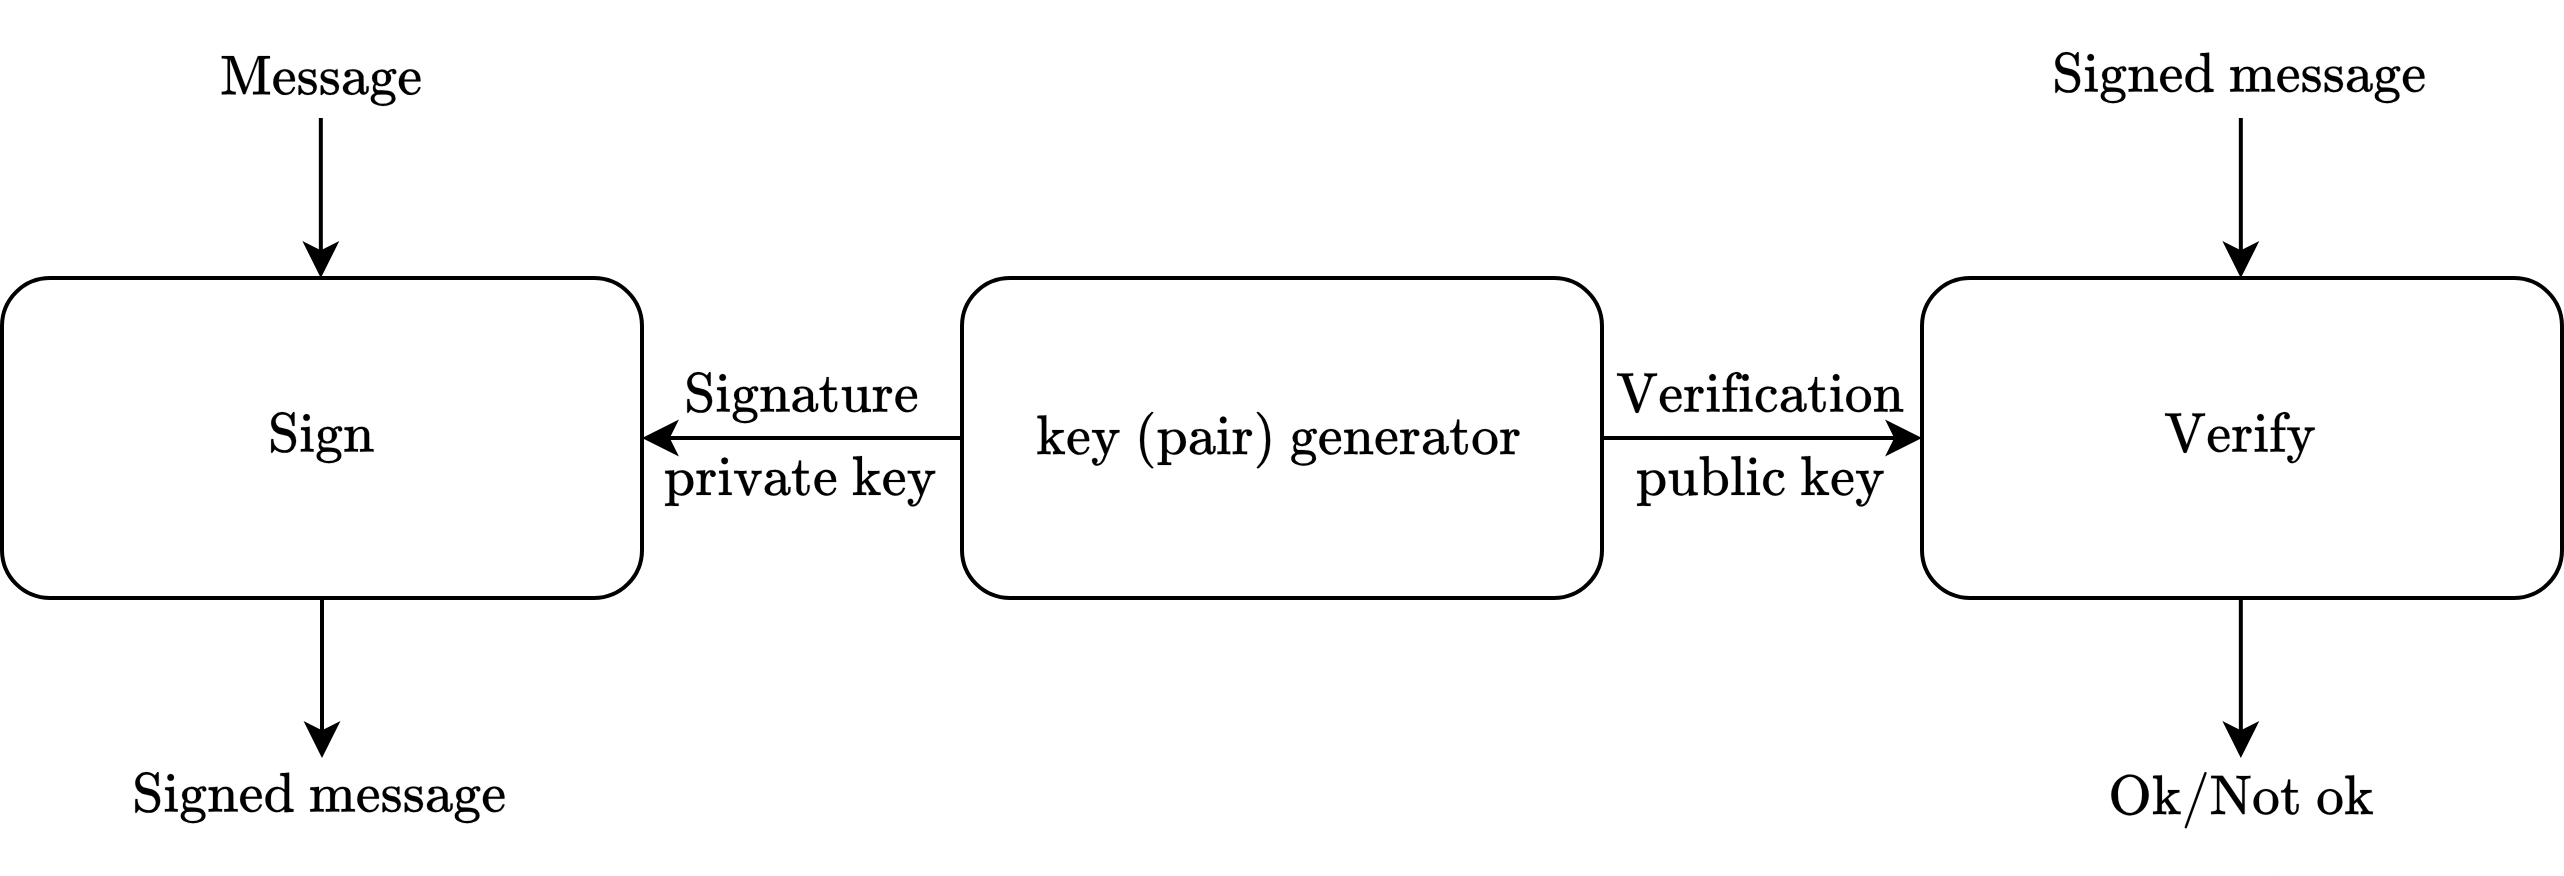
\includegraphics[width=0.75\linewidth]{images/aut.png}
    \caption{Digital signature}
\end{figure}
The computational challenges inherent in digital signatures encompass several key aspects:
\begin{itemize}
    \item Signing a message without possessing the signature key, which includes attempting to splice signatures from unrelated messages.
    \item Computing the signature key when provided only with the verification key.
    \item Attempting to derive the signature key solely from signed messages, without access to additional information.
\end{itemize}

\paragraph*{Algorithms}
In 1977, Rivest, Shamir, and Adleman (RSA) introduced a groundbreaking cryptographic method. 
This method employs a singular hard-to-invert function to craft both an asymmetric encryption scheme and a signature, with distinct message processing for each. 
Notably, the process of signing is significantly slower than verification, roughly around 300 times slower. 
This innovative approach has been standardized in NIST DSS (FIPS-184-4), underscoring its widespread adoption and importance in modern cryptographic practices.

The Digital Signature Standard (DSA) draws its foundations from adjustments made to signature schemes initially proposed by Schnorr and ElGamal. 
It, too, has been formalized in NIST DSS (FIPS-184-4), reflecting its establishment as a recognized cryptographic protocol. 
Notably, in DSA, the processes of signature creation and verification unfold at comparable speeds, distinguishing it from some other cryptographic methods.

\paragraph*{Usages}
Digital signatures serve various purposes:
\begin{itemize}
    \item \textit{Authenticating digital documents}: in order to enhance efficiency, digital signatures frequently entail signing the hash of a document rather than the document itself. 
        However, the assurance of the signature's reliability relies on the robustness of both the signature and hash algorithms.
    \item \textit{Authenticating users}: digital signatures present an alternative approach to user authentication, serving as a viable replacement for traditional password-based logins. 
        During this procedure, the server retains the user's public verification key, typically acquired during the account creation phase. 
        Upon authentication requests, the server initiates the client to sign a lengthy, randomly generated bit-string, referred to as a challenge. 
        Successful verification of the challenge signature by the client serves as compelling evidence of identity to the server.
\end{itemize}